\documentclass{beamer}

\usepackage{polski}
\usepackage[T1]{fontenc}
\usepackage[utf8]{inputenc}

\usepackage[polish]{babel}

\usepackage{subfig}
\usepackage{rotating}

%\usetheme[backgroundimagefile=bak.png,opacity=0.6]{diepen}

\usecolortheme{dove}
\setbeamertemplate{navigation symbols}{}

\setbeamertemplate{headline}{
	\vspace*{-1pt}
	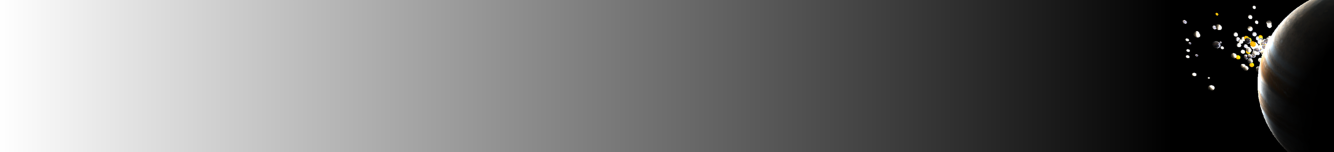
\includegraphics[width=\paperwidth]{bkg.pdf}}

\setbeamertemplate{frametitle}{
	\vspace{-1.6cm}
	\begin{overlayarea}{\linewidth}{1.6cm}
		\vfil\insertframetitle\vfil
	\end{overlayarea}
}
\setbeamerfont{frametitle}{shape=\upshape,series=\bfseries,size=\huge}

\title{Symulacja układu planetarnego na GPU przy użyciu CUDA i OpenGL}
%\subtitle{część druga}
\author{Daniel Kłobuszewski\and Jakub Kotur}
\institute{{\normalsize Promotor: Krzysztof Kaczmarski}\\\vspace{1cm} Politechnika Warszawska}
\date{\today}
%\logo{\includegraphics[height=0.5cm]{logo.png}}

\begin{document}

\frame{\titlepage}

\frame
{
	\frametitle{Treść prezentacji}
	\tableofcontents
}

\section{Założenia projektu}\label{sec:zalozenia}

\frame
{
	\frametitle{Założenia podstawowe}
	\begin{itemize}
	\item symulacja czasu rzeczywistego
	\item duże układy -- powyżej 10 000 planet
	\item dynamiczny silnik graficzny -- brak ładowania
	\item możliwie wydajny silnik fizyczny
	\end{itemize}
}

\frame
{
	\frametitle{Założenia dodatkowe}
	\begin{itemize}
	\item wygodne GUI
	\item zapis/odczyt układów
	\item symulacja układu słonecznego
	\end{itemize}
}
	

\section{Prezentacja programu}\label{sec:prezentacja programu}

\frame{\frametitle{Prezentacja programu}}

\section{Silnik graficzny}\label{sec:silnik graficzny}

\frame
{
	\frametitle{Rozwiązane problemy}
	\begin{itemize}
	\item dynamiczne wyświetlanie planet
	\item teksturowanie planet
	\item dynamiczne oświetlenie
	\item efekt atmosfer
	\end{itemize}
}

\frame
{
	\frametitle{Cele nie osiągnięte}
	\begin{itemize}
	\item komety -- zbyt skomplikowane
	\end{itemize}
}

\section{Silnik fizyczny}\label{sec:silnik fizyczny}

\frame {}

\section{Podsumowanie}\label{sec:podsumowanie}

\end{document}


